\documentclass{report}
\usepackage[utf8]{inputenc}
\usepackage[T1]{fontenc}
%\usepackage[italian]{babel}

%Disable all warnings issued by latex starting with "You have..."
\usepackage{silence}
\WarningFilter{latex}{You have requested package}
\pdfsuppresswarningpagegroup=1
%Bib
\usepackage[
backend=biber,
style=numeric,
citestyle=numeric,
]{biblatex}
\addbibresource{references.bib}

\usepackage{csquotes}
%\usepackage{natbib}


%Import
\usepackage{marvosym}
\usepackage{fancyvrb}
\usepackage[usenames]{color}
\usepackage[hidelinks]{hyperref}
\usepackage{url}
\usepackage{graphicx}
\usepackage{xcolor}
\usepackage{amsmath,amsfonts,amssymb,amsthm,mathtools}
\usepackage{caption}
\usepackage{enumerate}
\usepackage{multicol}
\usepackage{subcaption}
\usepackage{float}
\usepackage{indentfirst}
\usepackage{listings}
\usepackage{tocloft}
\usepackage[most]{tcolorbox}
\usepackage{pgfplots}
\usepackage{style/pgfplotsthemetol}
\pgfplotsset{compat=1.16}
\definecolor{lstgrey}{rgb}{0.94,0.95,1}
\lstset{
    backgroundcolor=\color{lstgrey},
    frame=single,
    rulecolor=\color{lstgrey}, % make frame "invisible"
    captionpos=t,
    tabsize=2,
    numberbychapter=false,
    showstringspaces=false,
    breaklines=true,
}
%LINK CLICCABILI
\hypersetup{
    colorlinks = true,
    linkcolor = .,
    citecolor = {blue},
    linkbordercolor = {white},
    urlcolor = {blue},
}
%TABELLE TBCOLORBOX
\tcbset{
        enhanced,
        colback=red!5!white,
        boxrule=0.1pt,
        colframe=red!75!black,
        fonttitle=\bfseries
       }



%PATH IMMAGINI
\graphicspath{{images/} {plantuml/rendered/} }
\newcommand{\emailaddr}[1]{\href{mailto:#1}{\texttt{#1}}}

\title{\LARGE
    MOTOSCALA
}

\author{
    Kiade Sara \\ \emailaddr{sara.kiade@studio.unibo.it}
    \and 
    Caminati Gyordan \\ \emailaddr{gyordan.caminati@studio.unibo.it} 
    \and 
    Giulianini Luca \\ \emailaddr{luca.giulianini2@studio.unibo.it}
    \and
    Ceroni Ruben \\ \emailaddr{ruben.ceroni@studio.unibo.it}
}

\date{August 2020}

\begin{document}
\maketitle
\tableofcontents

% -*- root: ../main.tex -*-
\begin{abstract}
Il problema del consenso rappresenta un elemento cruciale nei sistemi distribuiti, dove spesso diverse entità si trovano a dover concordare su un valore da assumere, al fine di convergere al medesimo stato. Nello specifico, il problema si presenta nel momento in cui si ha a che fare con \textbf{macchine a stati replicate}, dove la replicazione del dato deve mantenersi \textbf{consistente}.
Per portare a termine questo compito, sono attualmente disponibili diversi algoritmi di consenso.\newline
Il presente progetto consiste nello \textbf{studio approfondito e documentato} dell'algoritmo di consenso \textbf{RAFT} e delle sue applicazioni, arricchito da una implementazione che permette di evidenziare le sue peculiarità e di testarne il comportamento in diverse situazioni. Tale implementazione, infatti, fornisce un interfaccia utente tramite la quale è possibile agire su parametri significativi, al fine di poter eseguire agevolmente dei \textbf{test} e avere un riscontro degli effetti di questi ultimi sul \textbf{comportamento} del sistema.
\end{abstract}
% -*- root: ../main.tex -*-
\chapter{Introduzione}
L'obiettivo del progetto è quello di \textbf{sviluppare} un gioco arcade ispirato a \textbf{Motos}, avendo cura di mantenere un alto grado di \textbf{qualità} non solo nel risultato dell'\textbf{implementazione} ma anche in tutto ciò che riguarda il \textbf{processo di sviluppo}.
Per questo motivo tutti i \textbf{passaggi} che porteranno al risultato finale verranno \textbf{analizzati} con attenzione e \textbf{documentati} in maniera \textbf{dettagliata}.

\section{Il gioco} L'arcade \textbf{originale} consiste in un un \textbf{campo} bidimensionale sul quale il giocatore \textbf{pilota} una navicella e ha l'obiettivo di \textbf{eliminare} le entità nemiche spingendole \textbf{fuori} dal campo, \textbf{senza} essere eliminato a sua volta.

\textbf{MotoScala} replicherà gli aspetti principali del gioco originale, arricchendoli con l'inserimento di nuove \textbf{feature}, come il concetto di \textbf{durata vitale} delle entità e il \textbf{multiplayer}.

\section{Gli obiettivi}
Durante lo svolgimento del progetto si punterà al raggiungimento di \textbf{obiettivi} riguardanti il \textbf{processo di sviluppo}:
\begin{itemize}
    \item Rispetto delle \textbf{specifiche} non opzionali ed eventualmente integrazione di quelle aggiuntive.
    \item Utilizzo appropriato di tecniche \textbf{avanzate} di \textbf{gestione} del progetto.
    \item Rispetto degli standard di \textbf{qualità} introdotti a lezione.
\end{itemize}


% -*- root: ../main.tex -*-
\chapter{Processo di Sviluppo}
In questo capitolo verrano analizzati in dettaglio i processi relativi alle \textbf{metodologie di sviluppo} e \textbf{gestione di progetto} utilizzati. Per ogni processo inoltre, verrà fornita una breve descrizione di come esso sia stato \textbf{implementato} (tools, websites, ecc) e \textbf{automattizato} (CI).  
\section{Metodologia di Sviluppo}
Per quanto riguarda la metdologia di sviluppo scelta si è deciso di optare per un approccio moderno di tipo iterativo. Fra i tanti modelli presenti abbiamo scelto di mettere in pratica la metodologia \textbf{Agile} basata su \texttt{Scrum}. Data l'inesperienza nel campo del project managament abbiamo deciso di non scegliere una figura di \textbf{Scrum Master} in modo di avere un maggiore equilibrio decisionale. È stata invece definito il ruolo di \textbf{Product Owner}, svolto da Luca Giulianini, al quale è stato affidato il compito di \textbf{controllo qualità} e \textbf{validazione dei requisiti}.

\subsection{Scrum}
\label{subsec:scrum}
	\paragraph{Sprint} % (fold)
	\label{par:sprint}
	Gli \textbf{Sprint} hanno durata \textbf{settimanale} e, al termine di ognuno di essi, viene effettuata una \textbf{runione} generale di tutto il team al fine di \textbf{valutare i risultati} ottenuti. La riunione funge inoltre da \textit{strumento di confronto e dialogo} per quanto riguarda eventuali problemi emersi durante lo stesso Sprint. Una volta conclusa la riunione viene lasciata la parola al \textbf{Product Owner} il quale riassume brevemente lo stato attuale dello Sprint fornendo una breve \textbf{valutazione} circa la \textbf{qualità} dei \textbf{deliverables} prodotti e la loro aderenza ai \textbf{requisiti} precedentemente analizzati. Nel caso in cui vengano rilevate problematiche a livello qualitativo o di tempistiche, il team procederà a una ridefinizione del \textbf{piano di lavoro} modificando oppurtamente la \textbf{schedula} in modo da permettere un recupero graduale.
	% paragraph backlog (end)
	\paragraph{Backlog} % (fold)
	\label{par:backlog}
	Lo \textbf{Sprint Backlog} viene stilato dal team di settimana in settiama e alla fine di ogni Sprint, durante la consueta riunione generale, vengono valutati gli eventuali problemi aggiornando opportunamente il \textbf{Product Backlog}. Nel caso in cui uno Sprint venga completato con successo, il team procederà a incontrarsi nuovamente al fine di definire la documentazione relativa alla \textbf{nuova iterazione} e quindi il nuovo Sprint Backlog. Gli \textbf{items} del Product Backlog da introdurre nello Sprint sono \textbf{concordati} dall'intero team di sviluppo. Ogni item per comodità viene scomposto nei suoi \textbf{Sprint Tasks} di base e per ognuno di essi viene attribuito un valore di \textbf{effort} concordato dal team. Infine l'\textbf{assegnazione} dei task ai vari componenti del gruppo viene effettuata seguendo principalmente l'affinità con le \textbf{abilità} dei singoli membri del team.  
	% paragraph sprint (end)

\section{Gestione di Progetto}
Come abbiamo visto in \ref{subsec:scrum} la metodologia di sviluppo utilizzata è caratterizzata da una grande componente di \textbf{interazione} fra i membri del gruppo. Dato questo presupposto è fondamentale mettere in campo una serie di \textbf{tecnologie} e \textbf{strumenti} che permettano di semplificare questo processo. Al giorno d'oggi il mercato propone una serie di strumenti estremamente potenti e molti di questi vengono forniti gratuitamente a studenti universitari. Qui di seguito verranno elencati i tool utilizzati e verra fornita una breve descrizione delle loro peculiarità.

\paragraph{Trello} % (fold)
 Trello è un tool web di carattere manageriale basato sullo stile a Kanban. La struttura di una Kanban board è molto semplice: 
 \begin{itemize}
 	\item{\textbf{Colonne:}}
 	Rappresentano gli \textbf{stadi} di un determinato processo. Nella versione più semplice il processo segue tre semplici fasi: \textit{ToDo, Doing, Done }, mentre in ambito dello sviluppo software questo può introdurre al suo interno le fasi di sviluppo stesse come: \textit{review, backlog, doc, ecc}.
 	\item{\textbf{Cards:}}
 	Gli \textbf{items} in una Kanban board sono rappresentati da carte. Ogni carta contiene una serie di informazioni relative a un \textbf{task} come: \textit{durata, effort, ecc}.
 	\item{\textbf{Swimlanes:}}
 	In alcuni casi una Kanban board può essere integrata con il concetto di \textbf{Gantt Chart} connettendo così ogni singolo \textbf{task} a un determinato \textbf{membro} del team.
 \end{itemize}

\paragraph{Gantt Chart}
Il Gantt è stato molto utile nella fase di \textbf{assegnamento} dei vari task, esso permette infatti di poter fonire una stima temporale per ogni task permettendo così di avere un controllo totale sulla \textbf{schedula}. Inoltre unire il Gantt a un'approccio Kanban ci ha permesso di calcolare eventuali \textbf{ritardi} relativi ad ogni singolo task.

\paragraph{Github Project Management}
I \textbf{DVCS} negli ultimi anni sono passati dal-l'essere semplici gestori di codice a veri e propri gestori di progetto. \textbf{Github} è stato uno dei primi a partecipare a questa transizione e ha integrato nel tempo una serie di tool estremamente interessanti.
\begin{itemize}
	\item{\textbf{Organizzazioni:}}
	In Github c'è la possibilità di creare gruppi eterogenei facenti riferimento ad una organizzazione (reale o fittizia). Nel nostro caso è stata creata una organizzazione chiamata \texttt{Unibo-PPS-1920} che va a richiamare un \textbf{gruppo fittizio} dedicato al corso di Paradigmi di Programmazione e Sviluppo.
	\item{\textbf{Teams:}}
	Una volta definita una organizzazione è possibile creare all'inter-no di essa una serie di sottogruppi chiamati \textbf{teams}. Ogni team idealmente rappresenta uno \textbf{Scrum Team} costituito all'interno di una organizzazione o azienda con lo scopo di \textbf{portare a termine un progetto}. Il team dunque idealemnte dovrà attraversare tutte le fasi di costruzione, partendo da una prima fase di presentazione dei membri arrivando fino alla definizione delle \textbf{figure chiave} (Scrum Master, Product Owner). Nel nostro caso il team è stato nominato \texttt{CaminatiCeroniGiulianiniKiade} al fine di rispecchiare l'aspetto democratico dello stesso.
	\item{\textbf{Progetto:}}
	I progetti reali sono generalmente proposti dall'organizzazione (\textit{Senior Management}) e poi successivamente sono assegnati ai vari team. Nel nostro caso abbiamo voluto simulare questa situazione assegnando il progetto al team suddetto. Al fine di mantenere una corretta separazione di contenuti si è deciso di creare due progetti, uno dedicato agli \textbf{aspetti di documentazione} e l'altro dedicato agli \textbf{aspetti} meramente \textbf{implementativi}. I progetti sono sincronizzati tra loro attraverso  Trello e Github Projects.
	\item{\textbf{Projects:}}
	I Github Projects sono entità presenti all'interno dell'organiz-zazione e rappresentano una \textbf{interfaccia gestionale} sui vari progetti gestiti dall'organiz-zazione stessa. Nel nostro caso abbiamo definito un unico \textbf{Github Project} nel quale è stata implementata una piccola gestione di progetto a \textbf{livello operativo}. Al progetto infatti, sono delegati i compiti relativi alla gestione delle \textbf{Issues} e delle \textbf{Pull Requests} permettendo agli utenti di avere sotto controllo le \textbf{azioni} principali svolte dal \textbf{DVCS}.
\end{itemize}

\paragraph{Telegram}
Relativamente agli aspetti di \textbf{comunicazione informale} si è optato per uno strumento di messaggistica estremamente versatile, \textbf{telegram}. Grazie a Telegram e ai famosi telegram bots è stato possibile avere aggiornamenti diretti dal DVCS e CI consentendo un maggiore \textbf{controllo} su tutta la fase di \textbf{gestione e sviluppo} del progetto.

\paragraph{Discord}
Discord è stato utilizzando come strumento di \textbf{comunicazione} \textbf{se-mi-formale} \texttt{VoIP}. Su Discord è stato possibile chiarire dubbi e definire al meglio i task assegnati ai vari membri.

\paragraph{Teams}
Microsoft Teams è una piattaforma di comunicazione e collaborazione unificata che combina chat di lavoro persistente, teleconferenza, condivisione di contenuti. Come si può notare da questa definizione Teams è uno strumento di \textbf{comunicazione} estremamente \textbf{formale} ed è stato dunque utilizzato come \textbf{host principale} per le \textbf{riunioni Scrum}.

\paragraph{Notion}
Notion è un'applicazione a tutto tondo che fornisce supporto per quanto riguarda \textbf{gestione di task} e definizione di \textbf{ToDo lists}. È stata molto utile nella fase di \textbf{definizione} e \textbf{decomposizione} del \textbf{Product Backlog}.

\section{Continuous Integration}
Continuous
% -*- root: ../main.tex -*-
\chapter{Analisi dei Requisiti}

\section{Requisiti di Business}
\section{Requisiti Utente}
\section{Requisiti Funzionali}
\section{Requisiti non Funzionali}
\section{Requisiti Implementativi}
% -*- root: ../main.tex -*-
\chapter{Design Architetturale}
Dopo un'attenta analisi dei requisiti, si è proceduto con la fase di \textbf{design architetturale} che si è sviluppata in più passi, partendo dalla definizione ad alto livello di un'architettura generale e \textbf{raffinandola} gradualmente. 

	
\section{Architettura Generale}
Il primo passo per quanto riguarda l'aspetto della \textbf{progettazione} è consistito nella ricerca dei pattern più adatti da applicare, nell'individuazione dei principali componenti dell'\textbf{architettura generale}, e nella definizione dei modi in cui essi interagiscono.

La seguente immagine (fig: \ref{fig:architectureClassDiagram}) definisce il \textbf{core} dell'architettura generale che è stato successivamente \textbf{ampliato} per gestire anche la parte di architettura \textbf{client-server} necessaria alla realizzazione della modalità \textbf{multiplayer}.
\begin{figure}[H]
	\centering
	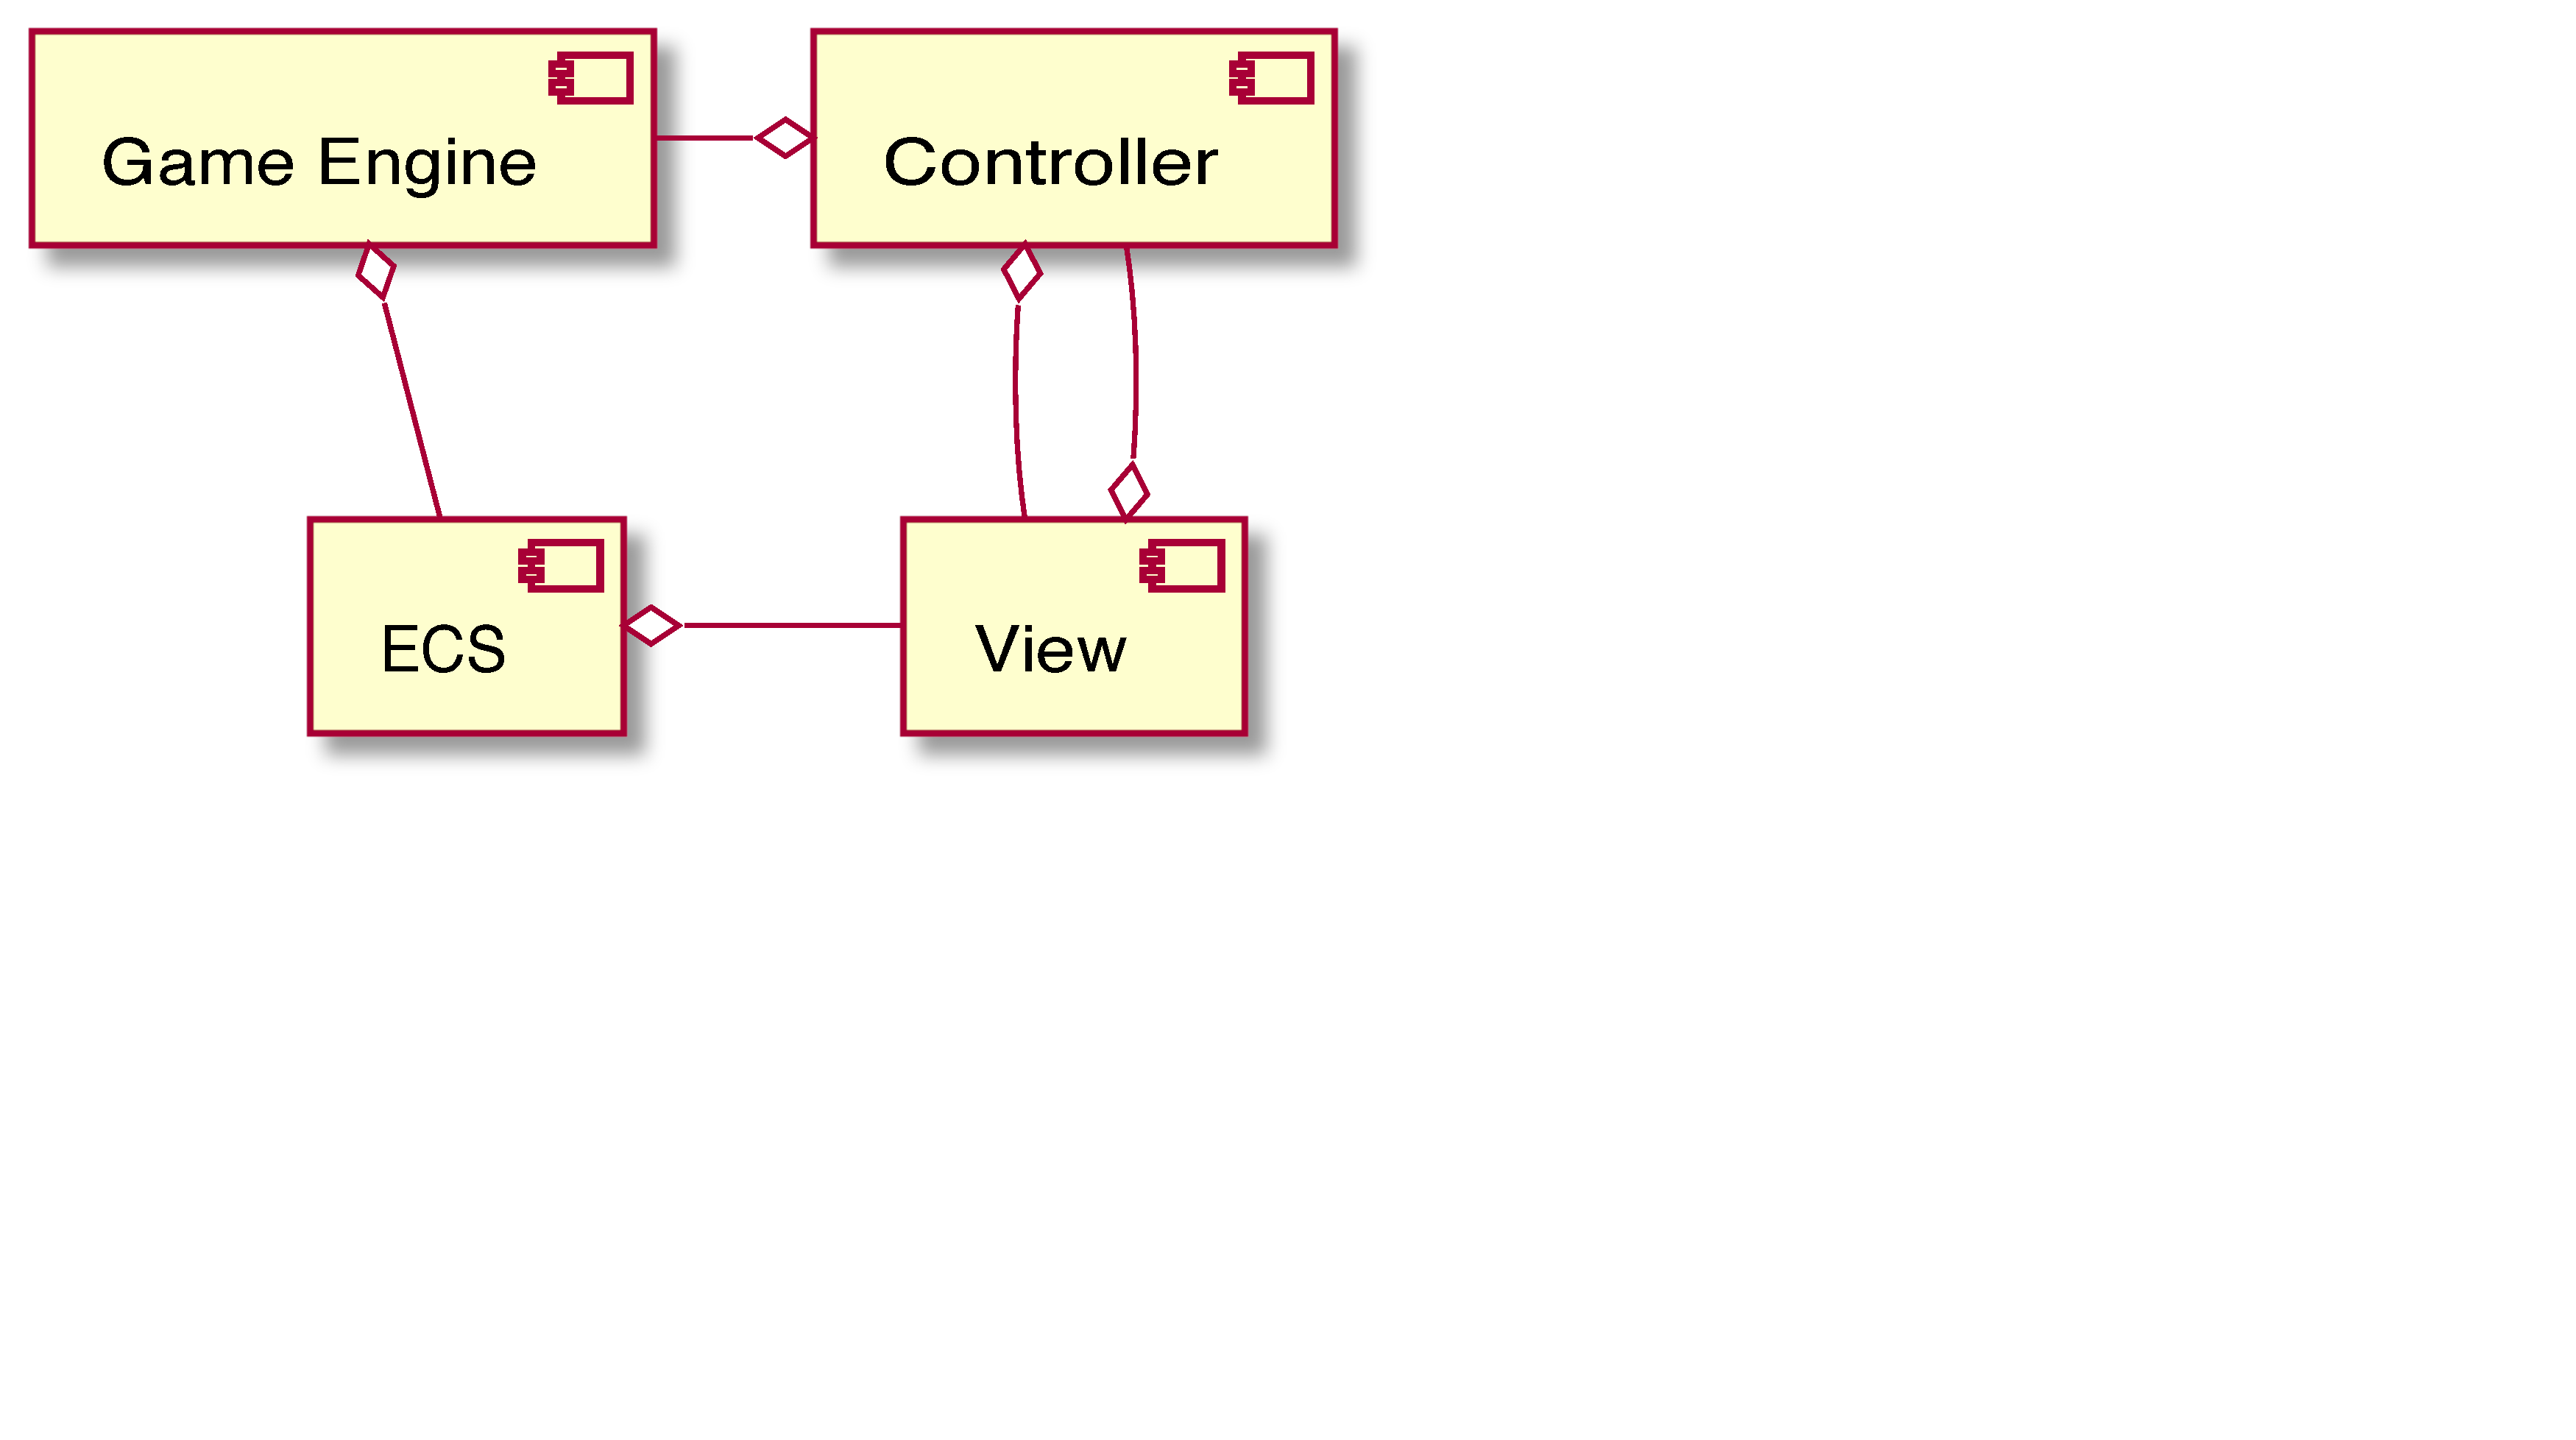
\includegraphics[width=0.80\columnwidth]{plantuml/rendered/classDiagrams/architectureClassDiagram.pdf}
	\caption{Diagramma raffigurante le entità principali dell’architettura e le loro interazioni ad un alto livello di astrazione.}
	\label{fig:architectureClassDiagram}
\end{figure}

Spiegazione breve delle entità in gioco

\begin{itemize}
    \item \textbf{View:} ha l'obbiettivo di fornire all'utente una \textbf{schermata} intuitiva per il controllo del gioco.
    \item \textbf{Controller:} rappresenta il punto di \textbf{snodo} per la gestione della logica principale dell'applicazione. La sua funzione primaria è quella di gestire la \textbf{comunicazione} tra: View, ECS, e GameEngine.
    \item \textbf{ECS:} è un aggregato di \textbf{sistemi}, \textbf{entità} e \textbf{componenti} che esprimono e contengono in maniera astratta la logica di gioco.
    \item \textbf{GameEngine:} rappresenta il cuore del gioco; incapsula il flusso di controllo principale e tramite ECS calcola continuamente il nuovo ambiente.
\end{itemize}

\section{Pattern Architetturali Utilizzati}
\subsection{ECS}
Trattandosi dello sviluppo di un videogioco, per il quale è necessario creare un motore di gioco, è stato scelto di utilizzare il pattern architetturale \textbf{Entity-Component-System} (ECS). Questo pattern è largamente utilizzato nello svi-luppo di videogiochi per motivi di performance e per la sua estensibilità e manutenibilità.

ECS si compone di tre parti principali:
\begin{itemize}
    \item \textbf{Entità:} rappresentano gli elementi in gioco, ad esempio Bumper car, PowerUp o Enemy. Ad ogni entità vengono associati uno o più componenti.
    \item \textbf{Componenti:} sono delle proprietà che vengono possedute da una o più entità e ne rappresentano lo stato. Esempi di possibili componenti sono direzione o posizione. 
    \item \textbf{Sistemi:} definiscono dei comportamenti necessari a gestire dei sottoinsiemi della logica di gioco. Gestiscono le interazioni tra le entità agendo sui componenti associati ad esse.
\end{itemize}


\subsection{MVC}
Il pattern \textbf{MVC} rappresenta uno standard per quanto riguarda il \textbf{design} di applicazioni \textit{robuste} ed \textit{estendibili}. Nel nostro caso il pattern è stato utilizzato in concomitanza con il pattern \textbf{ECS} permettendo così di raggiungere una maggiore \textbf{separazione dei concetti}. L'MVC progettato si compone dei seguenti moduli:
\begin{itemize}
    \item \textbf{Model:}
    All'interno del nostro applicativo esistono due tipi di modello:
    \begin{itemize}
        \item \textbf{Game Model:}
        Il \textbf{modello di gioco} rappresenta l'insieme delle \textbf{strutture dati} utili per modellare il gameplay. Nel nostro caso questo compito è stato catturato interamente dal \textbf{pattern ECS}.
        \item \textbf{Application Logic Model:}
        Il modello della  \textbf{logica applicativa} riguarda tutti i dati utili al \textbf{corretto funzionamento} dell'applica-zione (Impostazioni, Livelli, Dati utente, ecc).
    \end{itemize}
    \item \textbf{View:}
    L'interfaccia grafica si configura  come un \textbf{punto di intersezione} fra \textbf{ECS} e \textbf{MVC} per quanto riguarda gli aspetti dell'interazione utente. Essa si compone di due tipologie di schermate:
    \begin{itemize}
        \item \textbf{Game Screen:}
        È una schermata di gioco connessa interamente al modulo ECS. Essa ha come scopo principale quello di mostrare gli \textbf{aggiornamenti di gioco} e acquisire i \textbf{comandi} da parte dell'utente.
        \item \textbf{Application Screen:}
        È istanza di una semplice \textbf{schermata di presentazione}. Lo scopo di una application screen consiste essenzialmente nel garantire all'utente una buona \textbf{usabilità} e \textbf{interazione} col sistema, incapsulando le informazioni di modello in una \textbf{visualizzazione fruibile}. 
    \end{itemize}
    \item \textbf{Controller:}
    Gestisce le \textbf{interazioni} fra i principali moduli dell'architet-tura e mette a disposizione una serie di \textbf{funzionalità} relative alla \textbf{gestione delle risorse}.
\end{itemize}

\subsection{Client-Server} 
Un'architettura di tipo client-server si è resa necessaria per poter gestire la modalità di gioco \textbf{multiplayer}. Il sistema deve infatti permettere ad un utente di \textbf{ospitare} una partita assumendo il ruolo di \texttt{server} e ad altri utenti di \textbf{partecipare} ricoprendo il ruolo di \texttt{client}. 

\subsubsection{Scelta del paradigma}
Per gestire l'interazione tra Client e Server si è ritenuto adatto l'utilizzo del \textbf{paradigma ad attori} applicato mediante la modellazione di un attore \texttt{Server} e un attore \texttt{Client} che interagiscono tramite scambio di \textbf{messaggi}. 

\subsubsection{Distribuito vs centralizzato}
Quando ci si cimenta nella progettazione di un sistema che si interfaccerà in \textbf{rete} è necessario definire quale \textbf{approccio} utilizzare. Essenzialmente vi sono due strade percorribili: una basata su uno schema \textbf{centralizzato} mentre l'altra basata su uno schema \textbf{peer-to-peer}.
\begin{itemize}
    \item Approccio centralizzato
        \begin{itemize}
        \setlength\itemsep{0em}
        \item Semplicità
        \item Reattività
        \item Consistenza
        \item Single Point of Failure
    \end{itemize}
    
    \item Approccio distribuito
        \begin{itemize}
        \setlength\itemsep{0em}
        \item Fault-tolerance
        \item Carico suddiviso
        \item Modulare
        \item Complesso
        \item Incline all'inconsistenza
        
    \end{itemize}
\end{itemize}
Si è preferito utilizzare un approccio centralizzato anziché distribuito perché, data la natura del sistema che è da realizzare, si è ritenuto che una scelta diversa avrebbe portato, a fronte di un maggiore sforzo progettuale e implementativo, a dei risultati peggiori in termini di performance, reattività e consistenza.


Come mostrato dalla figura \ref{fig:clientServerComponentDiagram} il sistema è stato progettato in modo da poter estendere l'architettura core per il multiplayer, "staccando" l'engine del client e sostituendolo con l'attore client che poi comunicherà con l'attore server, che si interfaccia direttamente con il server.
\begin{figure}[H]
	\centering
	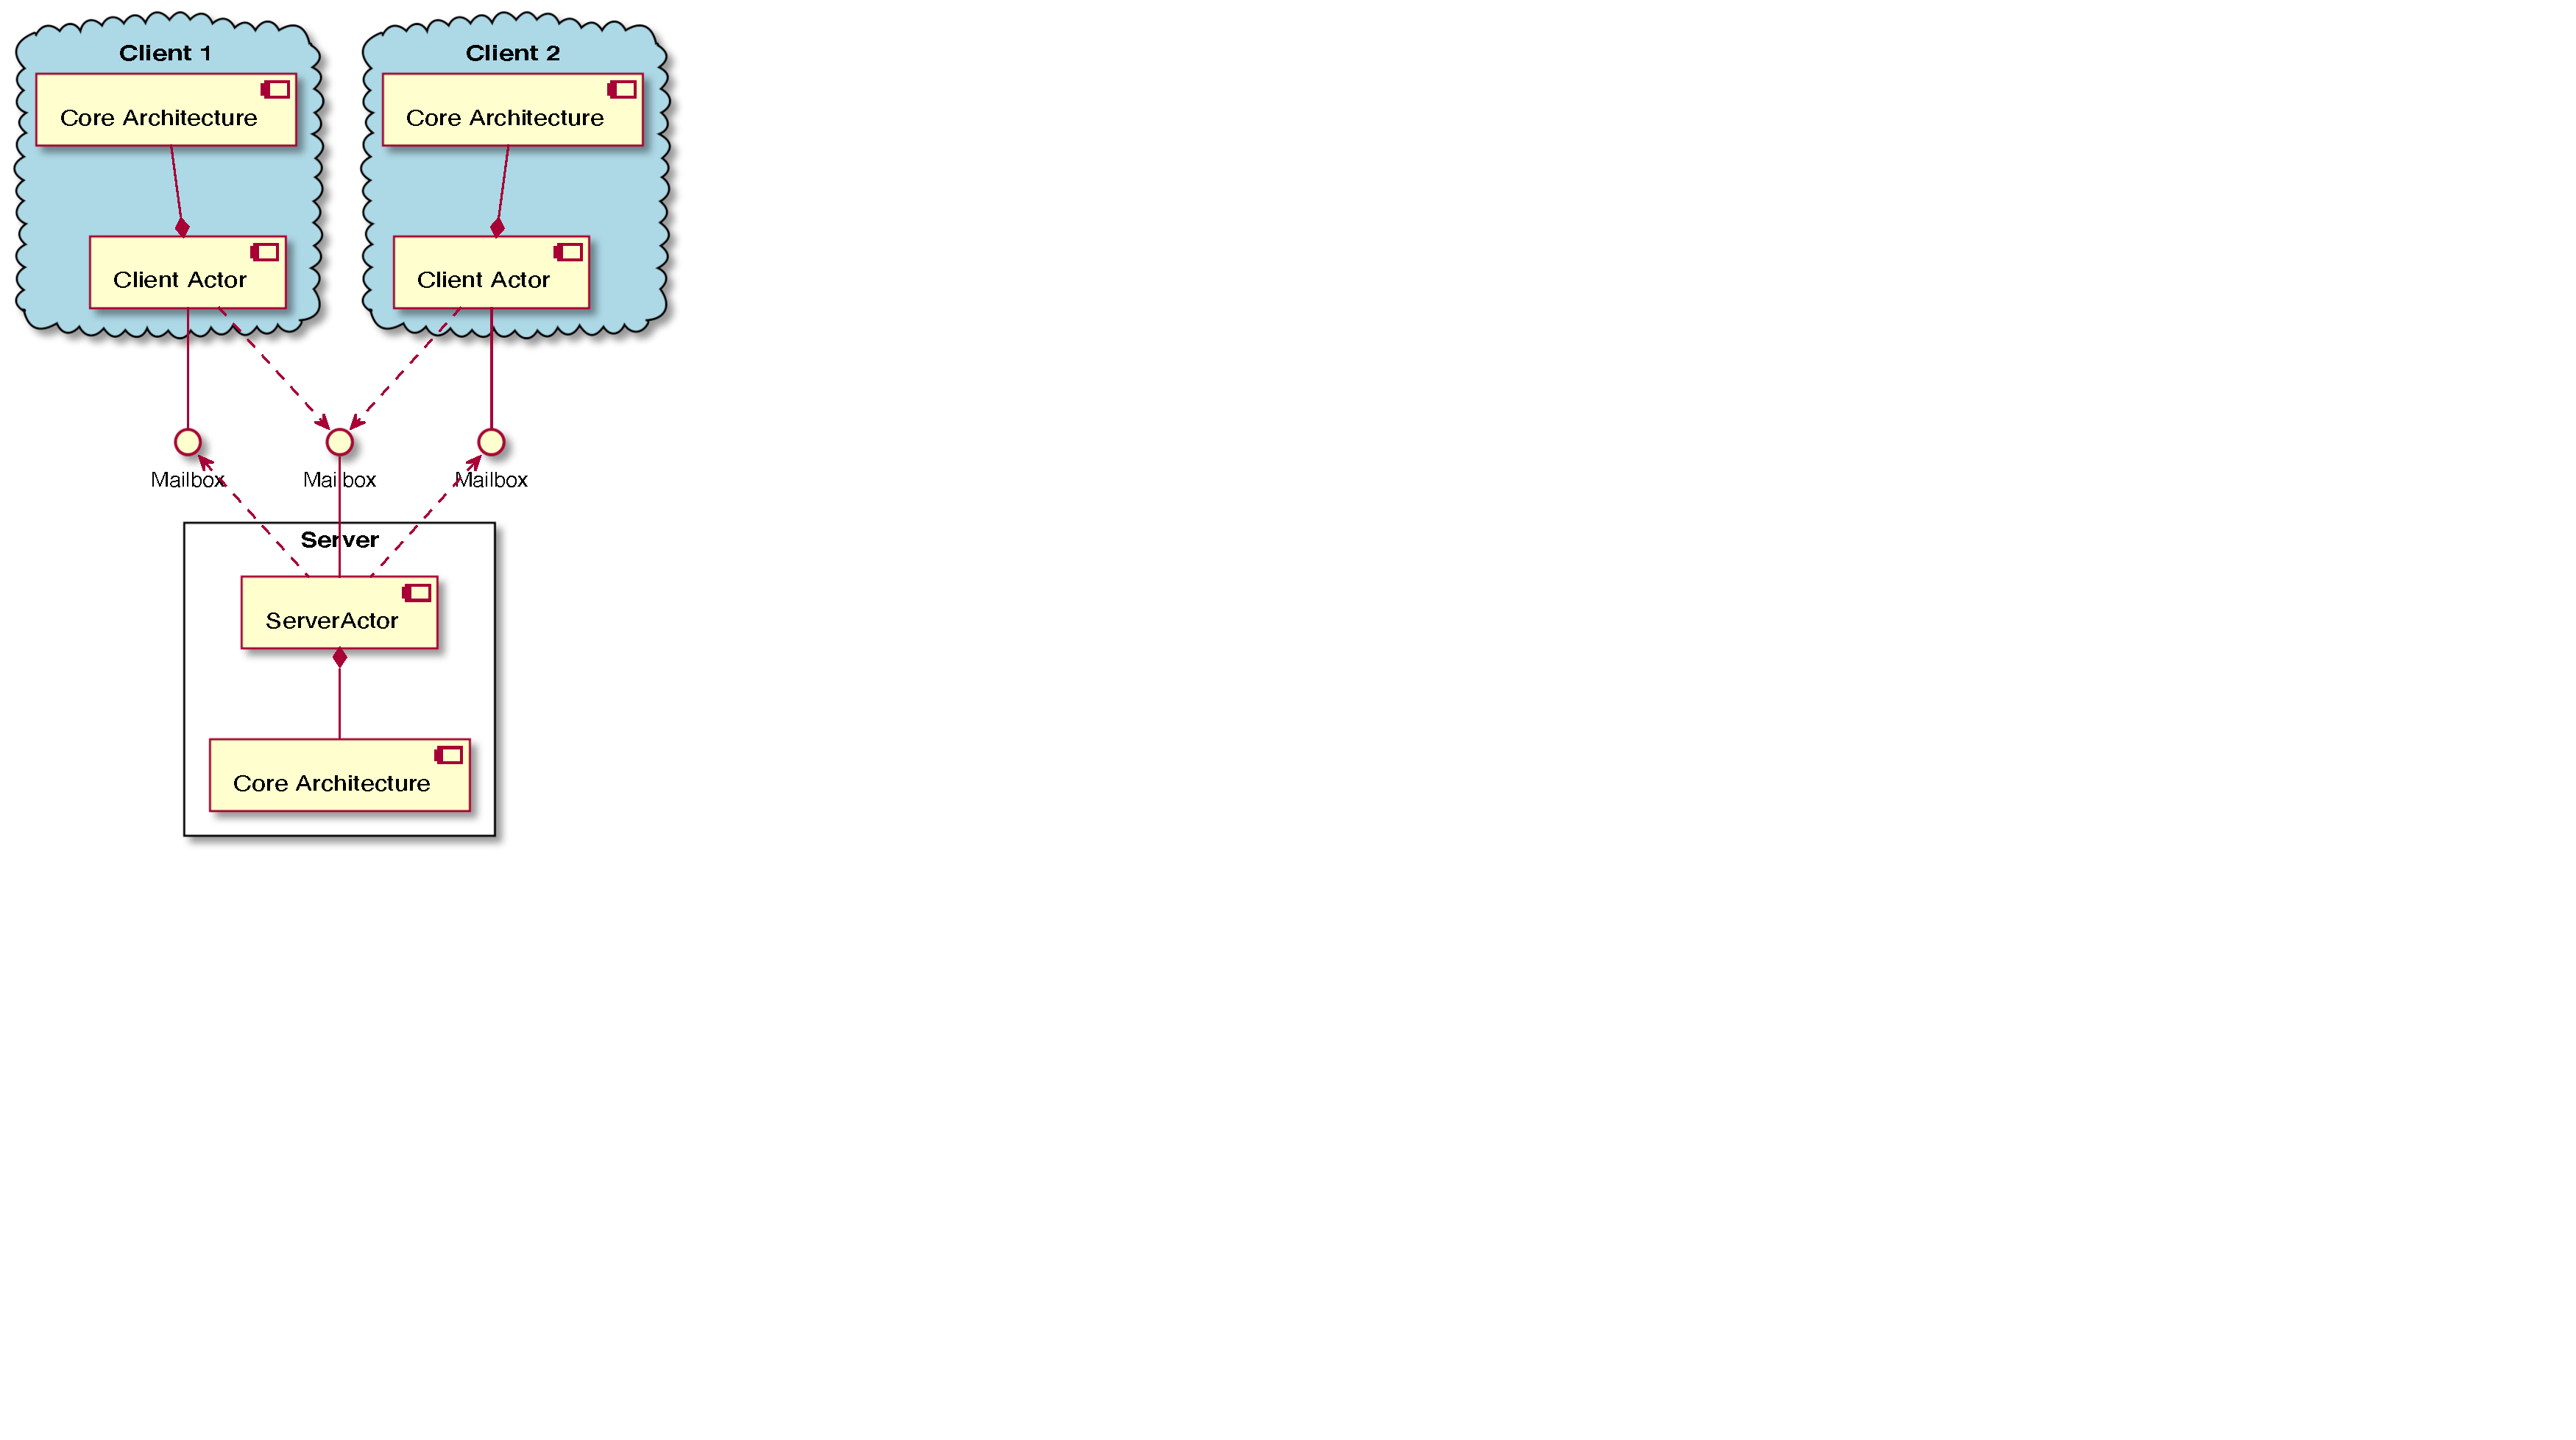
\includegraphics[width=0.70\columnwidth]{plantuml/rendered/componentDiagrams/clientServerComponentDiagram.pdf}
	\caption{Diagramma raffigurante gli attori di tipo Client e Server e le loro interazioni.}
	\label{fig:clientServerComponentDiagram}
\end{figure}

\section{Scelte Tecnologiche Cruciali}
    \subsection{Akka} 
        Per l'implementazione del paradigma ad attori sì e scelto di utilizzare \textbf{Akka} come layer di \textbf{comunicazione} nello sviluppo del multiplayer. Akka garantisce un'ottima \textbf{scalabilità} e un buon livello di \textbf{astrazione}, che permette di gestire la comunicazione in maniera più trasparente rispetto ai classici metodi basati sulle \textbf{socket}. Il modello \textbf{Client-Server} basato su Akka risulta così di facile \textbf{implementazione}.
        
        Inoltre, il fatto che Akka sia implementato in \textbf{Scala} rende più semplice e naturale l'utilizzo del framework. 
% -*- root: ../main.tex -*-
\chapter{Design di Dettaglio}
\section{ECS}
 %giustificazione ecs
 %Ogni sistema si occupa di gestire solamente uno o più componenti, aggiornandoli in blocco contemporaneamente. Questo approccio, in contrasto con l'approccio più OOP che consisterebbe nel modellare ogni entità come un oggetto, che deve implementare una sotto-interfaccia diversa in base al tipo, ereditando i metodi per l'aggiornamento. Questo causa problemi di performance all'aumentare delle entità da gestire, infatti ad ogni aggiornamento sarà caricato in cache l'intero oggetto e andrà recuperato dalla virtual table(TODO CHECK THIS) il metodo relativo all'aggiornamento. Ciò comporta un degradamento importante delle performance dato che gli accessi in RAM sono molto più lenti di quelli direttamente in cache. Sfruttando l'approccio ECS invece è possibile sfruttare meglio la cache, in quanto per ogni aggiornamento i componenti vengono caricati cache in blocco e processati dallo stesso metodo. 
\section{Scelte Rilevanti}
\section{Pattern di Progettazione}
\section{Organizzazione del Codice}
% -*- root: ../main.tex -*-
\chapter{Implementazione}

% -*- root: ../../main.tex -*-
\section{Luca Giulianini}
Lo studente Luca Giulianini si è occupato delle seguenti macro-parti:
\begin{itemize}
	\item{\textbf{Architettura generale e mediazione MVC-ECS}}
	\item{\textbf{Architettura ECS}}
	\item{\textbf{Architettura View}}
	\item{\textbf{Continuous Integration e configurazione dei Build-Tools}}
\end{itemize}

inoltre ha contribuito al lavoro dei colleghi svolgendo una serie di \textbf{micro-task}.

\subsubsection{Approfondimenti}

Parallelamente all'esperienza di progetto sono stati approfonditi una serie di argomenti relativi al mondo di \textbf{Scala} e della \textbf{programmazione funzionale}. 
\begin{itemize}
	\item{\textbf{Monadi:}} è stato chiarito il concetto astratto di \textbf{Monade}.
	\item{\textbf{Pogrammazione funzionale:}} è stato approfondito l'insieme delle \textbf{buo-ne pratiche} relative alla programmazione funzionale. Questo è stato fatto seguento svariate \textbf{conferenze} dedicate al mondo Scala e appoggiandosi a una serie di \textbf{libri} dedicati. 
	\item{\textbf{Refined Types:}} Molto utili nella fase di \textbf{validazione statica e dinamica} di input. Attualmente non utilizzati data la natura del progetto in questione.
	\item{\textbf{Monix e Akka Streams:}} È stato approfondito il mondo della programmazione \textbf{reattiva} focalizzandosi maggiormente sulle differenze fra il framework \texttt{Monix} e \texttt{Akka Streams}.
\end{itemize}

\subsubsection{Risorse}

Gli approfondimenti sono stati svolti grazie all'utilizzo delle seguenti risorse:
\begin{itemize}
	\item{\textbf{Libri:}}
	\begin{itemize}
		\item{\textbf{Learning Scala \cite{scalaLearning:2014}:}} libro che riassume interamente le \textbf{principali features} del linguaggio Scala in ambito \textbf{funzionale}. È stato usato per consolidare alcune conoscenze pregresse.
		\item{\textbf{Programming in Scala \cite{scalaBook:2014}:}} rappresenta la bibbia di Scala ed è stato scritto dal grandissimo \textbf{Martin Odersky}.
		\item{\textbf{Scala with Cats \cite{scalaCats:2020}:}} libro che copre gli aspetti più \textbf{avanzati} del linguaggio Scala dal punto di vista \textbf{funzionale}. Per ogni singolo aspetto è fornita una \textbf{definizione teorica} e la relativa implementazione nella libreria ufficiale \href{https://typelevel.org/cats-effect/}{\texttt{Cats}}. È un libro particolarmente \textbf{complesso} ed è stato utilizzato come approfondimento.
		\item{\textbf{Scala Cookbook \cite{scalaCook:2013}:}} I \textbf{Cookbook} di O'Reilly sono conosciuti per essere estremamente \textbf{pragmatici}. Anche in questo caso il libro si configura come un'\textbf{enciclopedia del problem solving} dedicata interamente al linguaggio Scala.
		\item{\textbf{Functional Programming in Scala \cite{functionalScala:2014}:}} davvero una grande scoperta. Questo libro rappresenta un insieme di \textbf{buone pratiche} e \textbf{aspetti teorici} che ogni programmatore Scala dovrebbe conoscere. Personalmente di grande utilità sono stati i capitoli che trattano la \textbf{gestione degli errori} e gli aspetti funzionali più avanzati (\texttt{monoids, monads} e \texttt{applicative functors}).  
	\end{itemize}
	\item{\textbf{Conferenze:}}
	\begin{itemize}
		\item{\textbf{Scala Days:}}
		Sono le conferenze ufficiali di Scala che ogni anno hanno luogo in un paese diverso. I talk proposti sono estremamente interessanti e permettono di apprendere un gran numero di \textbf{tecniche avanzate} e sopratutto costituiscono un ottimo esempio di \textbf{buona programmazione}.
		Conferenze consigliate:
		\begin{itemize}
			\item{\emph{\href{https://www.youtube.com/watch?v=CrpJJYPzdJE&t=630s}{Akka Streams to the Extreme - Heiko Seeberger}}}
			\item{\emph{\href{https://www.youtube.com/watch?v=pHHKUKubs1Q&t=2002s}{Migrating to Scala 2.13 by Julien Richard Foy and Stefan Zeiger}}}
			\item{\emph{\href{https://www.youtube.com/watch?v=DGa58FfiMqc}{Scala best practices I wish someone'd told me about - Nicolas Rinaudo}}}
			\item{\emph{\href{https://www.youtube.com/watch?v=I6pFxyL9Crc}{ScalaClean - full program static analysis at scale - Rory Graves}}}
			\item{\emph{\href{https://www.youtube.com/watch?v=TqJg4AuxEIQ}{Concurrent programming in 2019: Akka, Monix or ZIO? - Adam Warski}}}
			\item{\emph{\href{https://www.youtube.com/watch?v=_Rnrx2lo9cw}{A Tour of Scala 3 - Martin Odersky}}}
			\item{\emph{\href{https://www.youtube.com/watch?v=wfbF5jQiAhQ}{Security with Scala Refined Types and Object Capabilities by Will Sargent}}}
			\item{\emph{\href{https://www.youtube.com/watch?v=30q6BkBv5MY}{Functional Programming with Effects by Rob Norris}}}
		 \end{itemize} 
		\item{\textbf{Scalapeño:}} come dice il nome stesso, sono \textbf{conferenze piccanti} che hanno lo scopo di smuovere le acque all'interno della comunità di Scala.
		Conferenze consigliate:
		\begin{itemize}
			\item{\emph{\href{https://www.youtube.com/watch?v=v8IQ-X2HkGE}{The Last Hope for Scala's Infinity War - John A. De Goes}}}
			\item{\emph{\href{https://www.youtube.com/watch?v=Arwb6DSrWXE&t=102s}{Scala vs. Kotlin, friend or foe? - Ohad Shai}}}
		 \end{itemize} 
	\end{itemize}
\end{itemize}


\subsection{Architettura generale e mediazione MVC-ECS}
\subsection{Architettura ECS}
\subsection{Architettura View}
\subsection{Continuous Integration e configurazione dei Build-Tools}
\subsection{Micro-task}

% -*- root: ../../main.tex -*-
\section{Ruben Ceroni}


Lo studente Ruben Ceroni, conclusa la parte iniziale di analisi e progettazione comune si è concentrato sull'implementazione dei sistemi core del gioco e della loro integrazione con il resto del sistema.

\subsection{AISystem}
L'\texttt{AISystem} si occupa di generare gli spostamenti per le entità non controllate dal giocatore dotate di intelligenza artificiale e quindi di un AIComponent, nel quale è specificata la precisione dell'intelligenza artificiale e i possibili bersagli della stessa.

Il core della logica di movimento è stato implementato in \textbf{Prolog}, attraverso il predicato \texttt{move\_avoiding(+Q,+(SX,SY),+(TX,TY),+O,-DX,-DY)} che, prendendo in input una tupla (X,Y) di partenza e una di destinazione, fornisce in output il vettore direzione da prendere per arrivare alla destinazione.
La precisione è influenzabile tramite l'argomento Q, che esprime di quanto verrà falsata la posizione da raggiungere fornita in input.
L'array di posizioni O è necessario ad evitare che più nemici con lo stesso bersaglio si scontrino eccessivamente tra di loro inseguendolo.
La direzione risultante calcolata viene inserita nella stessa coda gestita dall'InputSystem che quindi gestisce lo spostamento delle entità nemiche allo stesso modo dei player.

\subsection{EndGameSystem}
L'EndgameSystem si occupa di monitorare lo stato della partita e di rimuovere le entità che escono dal bordo fornitogli in input o la cui vita abbia raggiunto lo 0 a causa delle collisioni subite.
All'eliminazione di un'entità  viene inviato tramite il mediator un \textbf{LevelEndEvent} contenente lo status della partita, l'entità eliminata e il punteggio ottenuto eliminandola.
Nel caso si tratti di un'entità nemica esso viene semplicemente rimosso dal gioco.
Mentre se si tratta di un'entità player o il player stesso rimane da solo in gioco, la partita viene considerata conclusa e viene stoppato l'engine, mentre lato view è mostrata la schermata di vittoria o di sconfitta. 
 
\subsection{PowerUpSystem}
Sono stati implementati 3 differenti tipi di powerUp.

L'attivazione di un powerUp è controllata dal \textbf{CollisionSystem}, che alla collisione di una entità player con un powerUp ne inserirà il riferimento all'interno del \textbf{PowerUpComponent} del powerUp.

Il comportamento specifico del singolo powerUp è specificato invece all'in-terno del suo \textbf{PowerUpEffect}, tramite una funzione che specifica come modificare il valore del componente modificato.

% \subsection{DrawSystem}

\subsection{Engine e GameLoop}
L'Engine rappresenta la parte core del gioco, e si occupa di istanziare i componenti principali e di registrare le entità del livello presso il Coordinator.
Il \textbf{GameLoop} è stato implementato come un thread separato che durante la sua esecuzione chiamerà il metodo tick dell'\textbf{UpdatableEngine} fornitogli in input, che porta all'aggiornamento di tutti i sistemi e la produzione di un frame di gioco. Per mantenere costante la frequenza di aggiornamento viene calcolato il tempo trascorso per produrre il frame e nel caso sia inferiore alla durata necessaria a mantenere gli fps costanti viene fatto attendere il thread.

\input{tex/implementation/sarakiade}
\section{Gyordan Caminati}

\section{Parti comuni}
\section{Aspetti Implementativi Cruciali}
% -*- root: ../main.tex -*-
\chapter{Retrospettiva}

\section{Processo di Sviluppo}
Durante le fasi iniziali di analisi dei requisiti e durante la Sprint 0 ci si è appoggiati al tool \textbf{Trello} per tenere traccia dei task da eseguire e degli artefatti prodotti.

In seguito, entrati nel vivo del progetto, si è deciso di utilizzare ai \textbf{Project} di \textbf{GitHub}, che mettono a disposizione un kanban virtuale come trello, ma completamente integrato con le issue di github e automatizzabile.


Una volta completata la fase iniziale e definiti gli item del backlog, essi sono stati inseriti in un \textbf{GitHub Project} relativo all'organizzazione GitHub creata per il progetto, consultabile all'indirizzo \url{https://github.com/orgs/Unibo-PPS-1920/projects/2}.

Sotto la stessa organizzazione sono stati creati sia il repository che contiene la relazione che quello contenente l'effettivo progetto.
Per ogni sprint è stato creato un nuovo github project in cui ddddddddddddddsono stati importati gli \textbf{item} del backlog relativi alla sprint dal project globale.

Questo approccio ha consentito di avere una visione pulita dello stato del progetto a livello alto e una visione più granulare a livello di sprint.

\section{Backlog}
Ogni item del backlog è stato formulato sotto forma di \textbf{User story}, dopo avere selezionato gli item da completare durante lo sprint planning, essi vengono tradotti in uno o più sotto-task implementativi.

\section{Iterazioni}
\subsection{Sprint 0}
A questo sprint è stato assegnato il numero 0 perchè non propriamente parte del processo di sviluppo iterativo, ma fondamentale per la produzione di solide basi per gli sprint successivi.
\subsubsection{Svolgimento}
Sono stati identificati i pattern architetturali applicabili e sviluppati in dettaglio i modelli delle parti principali del sistema


\subsection{Sprint 1}
\subsubsection{Svolgimento}
In questo sprint ci si è concentrati sul setup del progetto, in particolare di \textbf{Travis CI} e di \textbf{Gradle}, l'implementazione dello scheletro modellato nello sprint precendente.
In particolare sono stati implementati i componenti principali di ECS e il game engine.

\subsection{Sprint 2}
L'obiettivo di questa sprint è stato quello di mostrare una schermata all'uten-te con cui esso possa interagire.
\subsubsection{Svolgimento}
Lato view è stata sviluppata l'architettura principale MVC, il menu principale e il canvas.
Sono stati aggiunti i 3 system principali: InputSystem, DrawSystem e MovementSystem.
\subsubsection{Considerazioni}
Questo sprint è stato terminato con un leggero ritardo dovuto alla mole di lavoro necessaria a raggiungere l'obiettivo prefissatosi.
\subsection{Sprint 3}
L'obiettivo di questa sprint è stato quello di introdurre le feature mancanti dell'esperienza base del gioco.
\subsubsection{Svolgimento}
Sono state introdotte le componenti relative alla gestione degli scontri e l'intelligenza artificiale dei nemici, la gestione dei powerUp e la riproduzione dei suoni.
\subsubsection{Considerazioni}
Questo sprint si è rivelato più corposo del previsto, principalmente dovuto a un'astrazione non perfetta delle componenti di fisica, che hanno portato a un parziale redesign delle stesse all'introduzione del collision system.
\subsection{Sprint 4}
In questo sprint ci si è concentrati sull'aggiunta degli aspetti più avanzati come il multiplayer e sulla pulizia finale del codice
\subsubsection{Svolgimento}
È stato completato e rifinito il gioco. Sono state portate a termine la parte di integrazione con il multiplayer, la definizione dei livelli, l'aggiunta della durata vitale e del danno, il completamento e la revisione della documentazione, l'individuazione e la correzione di bug, il refactoring e la pulizia del codice. 

% -*- root: ../main.tex -*-
\chapter{Conclusioni}
Giunti alle conclusioni di questo progetto possiamo affermare di ritenerci estremamente soddisfatti del lavoro svolto. Il risultato ottenuto ha superato di gran lunga le nostre aspettative ma la strada che ha portato alla sua realizzazione è stata spesso impervia.\\
La realizzazione di un algoritmo di consenso richiede un enorme mole di studio e lavoro. Nel nostro caso il lavoro svolto si è suddiviso in questo modo: 
\begin{itemize}
  \item{\emph{Studio e documentazione:}}
  abbiamo impiegato all'incirca una settimana di lavoro al fine di comprendere e documentare al meglio l'algoritmo RAFT. Una volta che l'algoritmo è stato compreso si è potuto lavorare sull'effettiva implementazione concentrandosi inizialmente sulle varie tecnologie implementative. Dopo una breve indagine è stato scelto il framework Akka.
  \item{\emph{Studio di Scala:}}
  una volta che è stato individuato il framework di sviluppo, la scelta del linguaggio è stata quasi obbligata. Akka infatti, come abbiamo già visto, in Scala, permette di lavorare in modo estremamente conciso ed efficiente. L'apprendimento di Scala non è stato immediato e per comprenderlo al meglio abbiamo impiegato una settimana di studio full-time.
  \item{\emph{Studio di Akka:}}
  appreso il linguaggio Scala ci siamo concentrati sullo studio del framework Akka, in particolare ci siamo concentrati sulla libreria di Akka dedicata agli attori e al clustering.
  \item{\emph{Implementazione vera e propria:}}
  finalmente appresi i linguaggi e le tecnologie necessarie ci siamo concentrati sull'implementazione dell'algoritmo RAFT. Siamo partiti dal modello e abbiamo proseguito a sviluppare in modo incrementale i vari attori.
  \item{\emph{Debugging:}}
  completata l'implementazione l'algoritmo ha presentato un numero considerevole di bug. La fase di debugging è stata la fase più frustrante del progetto ma dopo grandi difficoltà siamo riusciti ad ottenere un'implementazione funzionante e pulita dell'algoritmo.
\end{itemize}


\section{Lavori Futuri}
  Il lavoro svolto come abbiamo visto è limitato a una semplice implementazione dell'algoritmo RAFT. Dato che l'algoritmo è stato sviluppato relativamente a un \textbf{caso d'uso specifico}, \textit{conti correnti bancari}, esso manca di estendibilità e genericità. Uno sviluppo futuro potrebbe risiedere nella possibilità di fornire una \textbf{versione generica} dell'algoritmo che sarà poi estendibile concretamente in base al caso d'uso.\\
  Un'altra possibile estensione futura dell'implementazione consiste nell'inserimento delle \textit{features extra} fornite dall'algoritmo RAFT: \textbf{Log Compaction} e \textbf{Configuration Changes}.

\section{Cosa Abbiamo Imparato}
  Quando si sceglie un progetto sostanzioso spesso si rischia di rimanere sommersi dal carico di conoscenze necessarie per portare a termine il lavoro. Nel nostro caso ci sono stati momenti di sconforto che, con supporto reciproco, siamo riusciti a superare. Gli argomenti che inizialmente si sono mostrati più ostici alla fine sono entrati a far parte del nostro bagaglio conoscitivo.
  \begin{itemize}
    \item{\emph{Scala:}}
    inizialmente abbiamo appreso solo le basi di questo linguaggio; il perfezionamento delle competenze è poi avvenuto in maniera passiva man mano che iniziavamo a far fronte ai diversi problemi che si presentavano. Questa esperienza ha avuto un impatto positivo: siamo entrati in contatto con un nuovo paradigma di programmazione, quello \textbf{funzionale}, e abbiamo imparato a lavorare in un ambiente OOP puro.
    \item{\emph{Akka:}}
    il framework Akka è sterminato e uno studio di un mese non basterebbe a coprire tutte le estensioni presenti. Nel nostro caso ci siamo concentrati solo sui moduli dedicati agli attori e al clustering e possiamo affermare che la conoscenza dei moduli è completa.
    \item{\emph{Algoritmi di Consenso:}}
    studiando RAFT abbiamo compreso il \textbf{funzionamento} e la \textbf{complessità} di un \textbf{algoritmo di consenso}, inoltre abbiamo toccato con mano la \textbf{complessità insita nelle interazioni fra entità nel distribuito}. Infine lo studio di RAFT ci ha permesso di entrare a conoscenza del fantastico mondo delle \textbf{macchine a stati replicate}.
  \end{itemize}

\clearpage

\section*{Note Stilistiche}
\begin{itemize}
  \item Le entità di progetto sono espresse in formato \texttt{Teletypefont}.
  \item Per gli indici e le variabili numeriche è stata usata la modalità \textit{math}. Es $n \in C$
  \item Gli spezzoni di condice sono espressi in formato \textit{listing}
  \begin{lstlisting}[language=bash]
echo ``Hello World''
  \end{lstlisting}
\end{itemize}

%\printbibliography

\end{document}
